\documentclass[11pt, twocolumn]{article}

\usepackage{url}
\usepackage{graphicx}
\usepackage{caption}
\usepackage{subcaption}

\def \gzipcompressionpct {30.63897}
\def \bzipcompressionpct {25.79215}
\def \beststrategypct {23.29247}
\def \bestdeltapct {71.15207}
\def \bestdeltaname {bsdiff comparing against the previous record}
\def \bestvsgzippct {76.02238}
\def \bzipvsgzippct {84.18089}
\def \domainscrawled {1,261}
\def \uniqueuris {63,179}
\def \requestssent {1,302,772}
\def \uniqueresponses {193,912}
\def \oldestpage {19 October 2008}
\def \youngestpage {06 December 2013}
\def \totaldays {1,874}
\def \iostarted {1,659}
\def \afterio {215}
\def \largewarccount {0}
\def \meanwarcsize {5,033,449}
\def \maxwarcsize {593,684,727}
\def \minwarcsize {4,352}
\def \newiasize {1.52045}
\def \newglaciercost {15,943}
\def \newglaciersavings {5,029}
\def \largestdomainname {beddebo-beddebo.github.io}
\def \largestdomaintotal {4,061}
\def \largestdomainmean {3,102}
\def \smallestdomainname {still3-still3.github.io}
\def \smallestdomaintotal {2}
\def \smallestdomainmean {2}
\def \meanfilechangesfirst {39.65521}
\def \meanfilechangeslast {595.92558}
\def \meandomainchangesfirst {2.71609}
\def \meandomainchangeslast {15.00000}
\def \referenceframeoverhead {5.46623}
\def \bsdifffirstoverhead {4.27673}
\def \warcfilecount {1,261}
\def \productionwarcfilecount {6}
\def \meanresponsesize {18042.12673}
\def \meanresponsemultiplier {24}
\def \meanresponsebsdiffimprovement {}
\def \meanresponsebsdiffsize {}
\def \meanresponsebsdiffmultiplier {}

\begin{document}

\section{Introduction}

  Web archiving initiatives generate vast amounts of data. The Internet Archive advertise their collection to be almost 2 petabytes, growing at a rate of 20 terabytes per month\footnotemark. The cost of providing storage for large collections can be high. For instance Amazon's Glacier service, an ``extremely low-cost storage service'', advertise storage rates of \$0.01 per GB per month as of February 2014. At this rate The Internet Archive would pay \$20,972 per month. Requests to browse the archive would incur additional costs, as would expanding the archive. This situation motivates us to ask how web archive data can be compressed in order to optimally reduce storage space.

  The Web ARChive (WARC) file format is the ISO standard\footnotemark commonly used to store web archive data. It is a plain text format that contains records of requests and responses made to URLs. When building a web archive that spans many domains, the standard recommends appending records to WARC files until they reach 1 gigabyte, uncompressed. At this point they should be gzipped and stored. Using this recommendation our data set from Section~\ref{section:exp:github} compresses down to $\gzipcompressionpct\%$ of its original size. The WARC file format is extensible and the standard lists possible compression extensions. To our knowledge no such extension has been made publicly available and none are widely used. In this paper we explore possible extensions to the WARC format that would allow delta compression of consecutive records as well as different compression algorithms. We aim to: (i) reduce the total archive size and, (ii) allow easy partitioning of the archive. The strategy that leads to the smallest total archive size compresses down to $\beststrategypct\%$ of the original. Applying our strategy to the Internet Archive's collection would reduce their collection down to $\newiasize$ petabytes and their (hypothetical) Amazon Glacier costs to $\$\newglaciercost$ per month, a saving of $\$\newglaciersavings$.

  \footnotetext{\url{https://archive.org/about/faqs.php#9}}
  \footnotetext{\url{http://www.iso.org/iso/catalogue_detail.htm?csnumber=44717}}

\section{Background}

  \begin{enumerate}
  \item WARC spec
  \item gzip, bzip2, tar. What they do, why these ones?
  \item vcdiff, bsdiff, diffe. What they do, why these ones?
  \item internet archive, IIPC, BL. Collections, experience
  \item Heritrix
  \end{enumerate}

\section{Experiment: Generated Data}

  \begin{enumerate}
  \item generate 1MB text data
  \item apply change repeatedly
  \item compression strategy
  \item compare
  \item very many changes, over time. What wins
  \item More than just text data? What kinds of changes?
  \end{enumerate}

\section{Experiment: GitHub Pages}\label{section:exp:github}

  The code hosting service GitHub\footnotemark offers a free service called GitHub Pages\footnotemark that hosts users' static web content for free. Each web site is stored in a Git repository, also hosted by GitHub. In order to evaluate different compression strategies on realistic data we downloaded $\domainscrawled$ GitHub Pages repositories. As these web sites are stored in version control it is possible to iterate through the changes made to the files over time. Doing this we can repeatedly crawl a web site as changes are made to it. We can then explore how different compression strategies perform. In particular we are interested in the total size of the archive after compression.

  \subsection{Data}

    The data set is made up of repositories hosted on GitHub that conform to the projectname.github.io naming scheme. GitHub treats these repositories as GitHub Pages repositories and serves their content at the URL given by the name (i.e. http://projectname.github.io). When changes are pushed to the repository the files and website are updated. Before hosting, the files are processed by a static website generator called Jekyll\footnotemark. To generate our data set we clone a repository and iterate through every commit. For each commit we process the files using Jekyll and serve the results up locally. We then direct Heritrix to archive the site. When Heritrix has finished we stop serving and continue to the next commit. When we have processed an entire repository we tidy up the WARC files that Heritrix has produced to make sure they conform to the guidelines in the WARC standard. In particular we replace any identical response records coming from the same URI with a revisit record. We also combine uncompressed WARC files until they reach a maximum of 1 gigabyte in size.

    During this process we have crawled $\domainscrawled$ domains, discovering $\uniqueuris$ URIs. Heritrix sent $\requestssent$ requests for pages and received $\uniqueresponses$ unique responses. Our archived data spans $\totaldays$ days, from \oldestpage{} to \youngestpage.

    % TODO: Using version control language, need to define? e.g. clone, push

    \footnotetext{\url{http://github.com/}}
    \footnotetext{\url{http://pages.github.com/}}
    \footnotetext{\url{http://jekyllrb.com/}}

  \subsection{Compression Analysis}

    We now explore different strategies for minimising WARC file size using compression and delta algorithms. We compare two compression algorithms; gzip and bzip2, we also consider tar files that use these compression types. When compressing without tar, we treat each WARC file individually. With tar we combine all WARC files under a single domain into a tar file and then apply the compression algorithms. When applying a delta algorithm we consider every response record in a WARC file, choosing, if applicable, a second response record to compare against. We replace these response records with revisit records, the payloads of which contain the patches that can be used to re-create the original record. When choosing the response record to compare against we use three strategies. In one we compare against the first record ever recorded for that URI. In the second we compare against the record that was most recently recorded for that URI. In the third we compare against reference records that are stored every ten responses.

    Storage restraints meant that we could not consider every domain at once, instead we consider each in turn. This means that each WARC file contains only records from a single domain. It also means that few WARC files exceed the 1 gigabyte size limit. In fact $\largewarccount$ WARC files exceeded the one gigabyte limit. In archiving our $\domainscrawled$ domains we created $\warcfilecount$ WARC files. In a production system these files would have been concatenated and stored in $\productionwarcfilecount$ files. The larger a file, the more data a compression algorithm has to work with, we believe that this may increase the size of our compressed archive over the production. However, because we store all domain related material in the same file we believe that compression algorithms have a higher quality of data to work with. This would have the effect of decreasing our compressed archive size over a production system. In a seminar in 2013 the British Library stated that their recent archiving initiatives were stored compressed down to roughly 40\% of the original size. Our gzip compression reduces our archive down by $\gzipcompressionpct\%$, we believe that this indicates that our results are similar enough to a production archive to be generalisable. The largest WARC file is $\maxwarcsize$ bytes, the smallest $\minwarcsize$, the average WARC file is $\meanwarcsize$ bytes.

    Figure~\ref{fig:tas_delta_compression:a} shows the total archive size for different compression algorithms. The WARC specification recommends that files are compressed using gzip. Applying this strategy to our archive compresses the files down to $\gzipcompressionpct\%$ of the original. We see that applying a bzip2 algorithm would compress the archive down to $\bzipcompressionpct\%$. Figure~\ref{fig:tas_delta_compression:b} shows the effect of applying delta algorithms to the data. The best performing delta strategy uses bsdiff to calculate the delta between each consecutive record. Using this strategy we see a $\bestdeltapct\%$ reduction in total archive size. Figure~\ref{fig:tas_best} shows the total archive size attainable when using a combination of delta and compression algorithms. By applying a delta algorithm to the response records and then compressing the resulting files we can further reduce the total archive size. We see that if we apply the vcdiff algorithm to each consecutive record and then compress everything using bzip2 we can reduce the total archive size to $\beststrategypct\%$ of the original. This best performing strategy produces a collection $\bestvsgzippct\%$ of the size of that of the recommended compression strategy.

    \begin{figure}
      \centering
      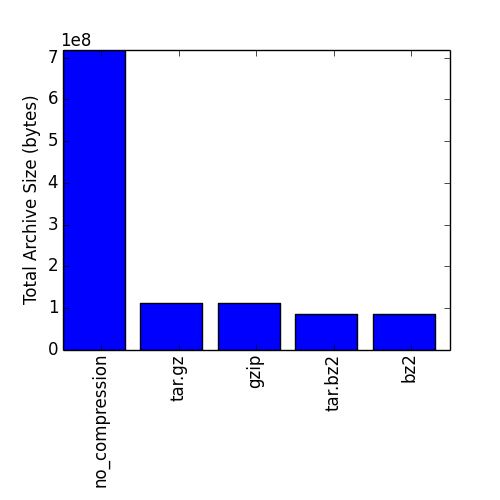
\includegraphics[width=\linewidth]{images/tas_compression.png}
      \caption{Compression comparison.}
      \label{fig:tas_delta_compression:a}
    \end{figure}
    \begin{figure}
      \centering
      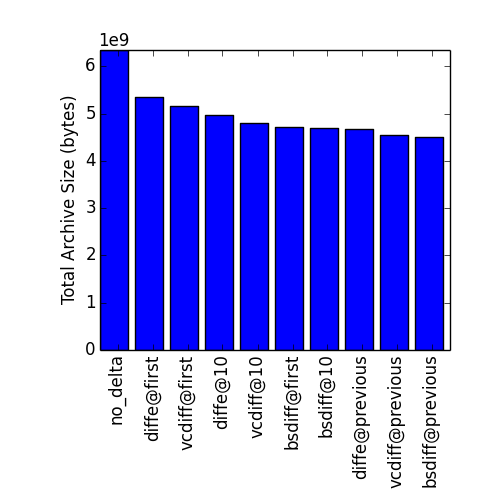
\includegraphics[width=\linewidth]{images/tas_delta.png}
      \caption{Delta comparison.}
      \label{fig:tas_delta_compression:b}
    \end{figure}
    
    \begin{figure}
      \centering
      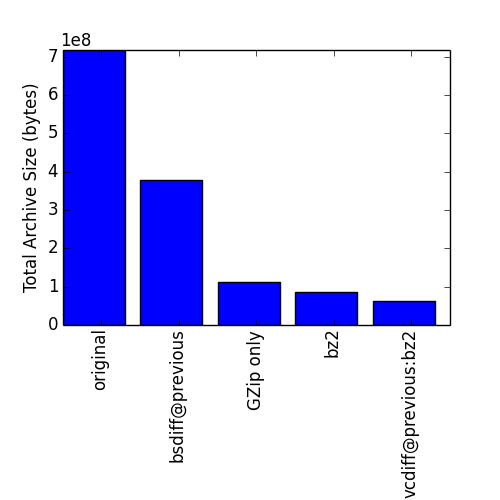
\includegraphics[width=\linewidth]{images/tas_best.png}
      \caption{Total archive size for different delta and compression strategies.}
      \label{fig:tas_best}
    \end{figure}

    We see above that the bzip2 compression algorithm produces a smaller archive than gzip, in our direct comparison bzip2 compresses our data set down to $\bzipvsgzippct\%$ of the size of gzip. In fact, bzip2 tends to more optimally compress data than gzip in many benchmarks\footnotemark. However, those benchmarks show that bzip2 can be slower than gzip (in one benchmark, 4.5x slower to decompress compressed data). In a web archive setting, where long-term storage is a high priority, we believe that bzip2 is the better choice of compression algorithm. The space savings it provides can be significant when considering the scale of an archive and the increased access time will be of negligible cost to the archive owner. When comparing delta algorithms we see that calculating the delta between a record and the immediately preceding record produces the smallest archive, no matter the delta algorithm. This is to be expected as it is likely that consecutive records will be quite similar in the majority of cases, producing smaller deltas. The downside to this strategy is that recreating a record requires access to every preceding record, each must be patched in turn. As a solution to this problem we introduced a reference frame every 10 records that is stored in full. Each record is compared to its closest preceding reference frame, recreating a record requires access to, at most, 10 previous records. Using reference frames introduces overheads, on average the archive size increased by $\referenceframeoverhead\%$ when compared to strategies using immediately preceding records. A second alternative delta strategy is to compare every record to the first record ever recorded for a URI. In this case every record can be recreated using only one previous record (the first). We would expect this strategy to under perform because as changes are made to the file the delta between it and its original must get more complicated. This is the case for the diff and vcdiff algorithms, surprisingly bsdiff produces a smaller archive when comparing to the first record than when it compares to the reference frame. Using the bsdiff algorithm to produces deltas between a record and the first record creates an archive $\bsdifffirstoverhead\%$ larger than that created when comparing to the previous record.

    % bsdiff does better but can't be compressed as well.
    % put vcdiff@previous, bsdiff@previous and bsdiff@first on graph
    % generally what's better vcdiff or bsdiff?

    \footnotetext{e.g. \url{http://compressionratings.com/sort.cgi?txt1.brief+4np2}}

    Figure~\ref{fig:record_type_size} shows the mean size of each record type in our archive. For response records we also show the mean size after a delta strategy has been applied. The response records take up the majority of a WARC file. Without delta, the mean response record is $\meanresponsesize$ bytes, $\meanresponsemultiplier x$ the next largest record type, metadata. With bsdiff applied to response records the mean size drops by $\meanresponsebsdiffimprovement\%$ to $\meanresponsebsdiffsize$ bytes, $\meanresponsebsdiffmultiplier x$ the mean metadata size.

    \begin{figure}
      \centering
      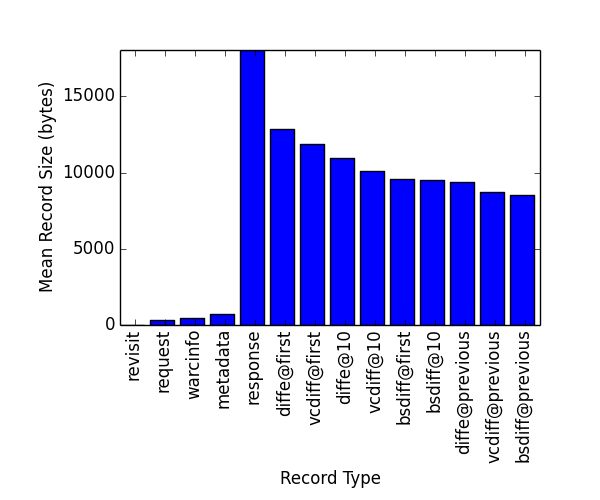
\includegraphics[width=\linewidth]{images/record_type_mean_size.png}
      \caption{Size of records in WARC file by record type.}
      \label{fig:record_type_size}
    \end{figure}

    \begin{enumerate}
    \item what are the pros and cons of each strategy. e.g. speed, partitioning, do we gain little over the other strategies in terms of size but lose on speed?
    \item additionally:
    \begin{enumerate}
    \item savings introduced by compression, why not compress the other types?
    \item compression performance by content type
    \item refer to content analysis for frequencies of content type. e.g. is it worth finding an algorithm that compresses images really well? or can we ignore them because HTML and its high change frequency trump image for storage issues.
    \end{enumerate}
    \end{enumerate}

  \subsection{Content Analysis}

    Figure~\ref{fig:file_changes_per_day:a} shows the number of files that changed in the archive per day. The data is split into two parts for clarity. The split is made on the day that GitHub pages launched their new naming scheme, projectname.github.io on 5 May 2013. Previously the naming scheme had been projectname.github.com. Our data crawl did not consider projects that had kept the old naming scheme. In the first $\iostarted$ days the mean number of files changing per day was $\meanfilechangesfirst$, in the last $\afterio$ that increases to $\meanfilechangeslast$.

    % TODO: Insert more meaningful analysis of change frequency. Is there a strong correlation? Can we say something like 'the average domain will update at least one page every X days'? DO we see an increase in change frequency over time? Is this explained by an increase in suitable projects over time? Can we correct for this?

    \begin{figure}
      \centering
      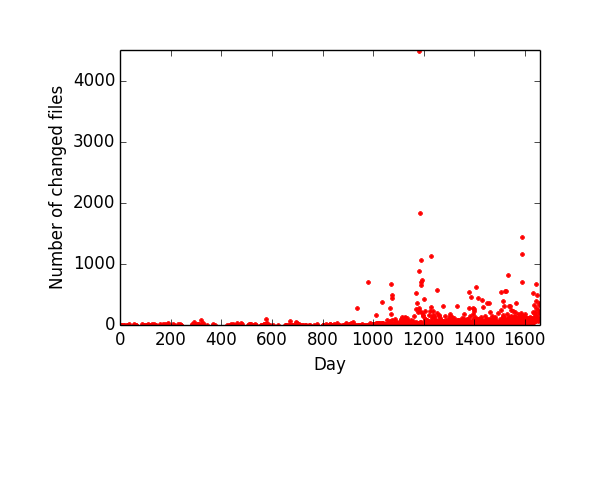
\includegraphics[width=\linewidth]{images/file_changes_per_day_first.png}
      \caption{Changes during the first \iostarted{} days.}
      \label{fig:file_changes_per_day:a}
    \end{figure}
    \begin{figure}
      \centering
      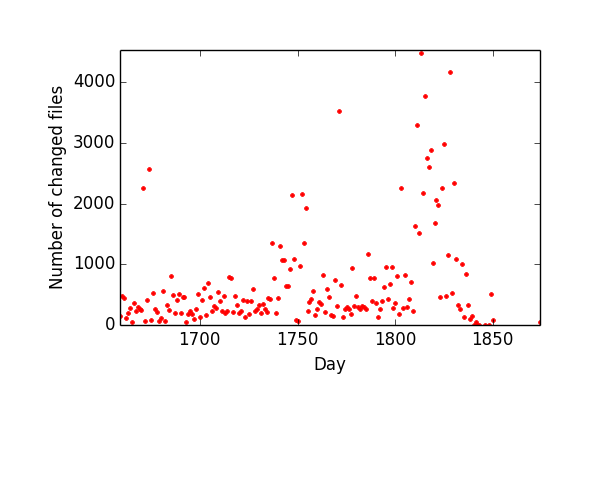
\includegraphics[width=\linewidth]{images/file_changes_per_day_last.png}
      \caption{Changes during the last \afterio{} days.}
      \label{fig:file_changes_per_day:b}
    \end{figure}

    Each file change is an observation of a single file's contents differing from a previous crawl. This means that if a HTML file and a CSS file were updated simultaneously, we would record two changes. This might not align with an archivist's view of what a webpage change would be. Instead, they might expect to record a single change for updates made in a short period of time, no matter how many files were edited. In addition, we iterate through every commit made to the project but changes are only made public for every push. There may be several commits made to a project before a push. Considering this, we can instead assume that a maximum of one change is made to a domain per day. Figure~\ref{fig:domain_changes_per_day:a} shows the number of domains that change in the archive per day. During the first segment we see a mean of $\meandomainchangesfirst$ domains changing per day, in the second segment this is $\meandomainchangeslast$.

    \begin{figure}
      \centering
      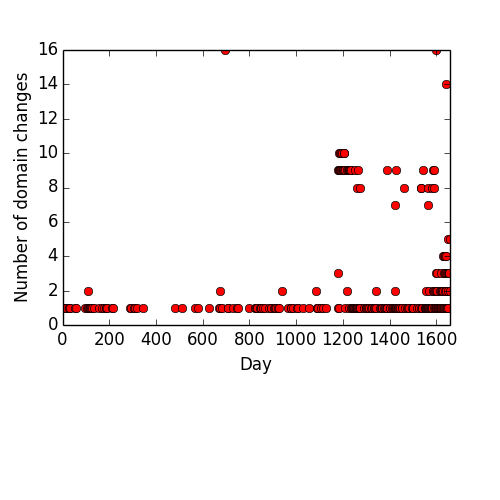
\includegraphics[width=\linewidth]{images/domain_changes_per_day_first.png}
      \caption{Domain changes during the first \iostarted{} days.}
      \label{fig:domain_changes_per_day:a}
    \end{figure}

    \begin{figure}
      \centering
      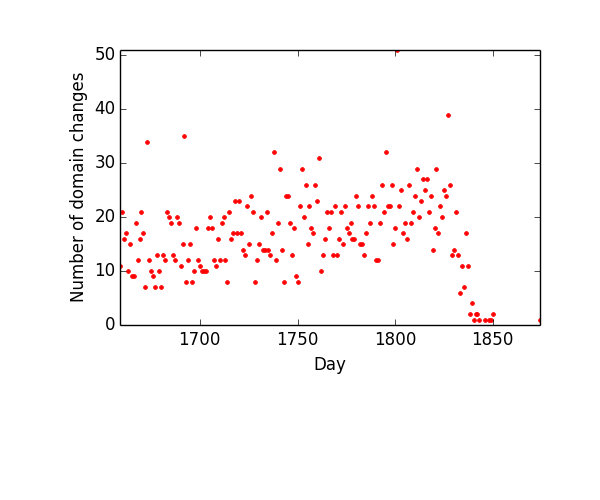
\includegraphics[width=\linewidth]{images/domain_changes_per_day_last.png}
      \caption{Domain changes during the last \afterio{} days.}
      \label{fig:domain_changes_per_day:b}
    \end{figure}
    
    Figure~\ref{fig:uris_per_domain:a} shows the total number of URIs ever observed at a domain. Figure~\ref{fig:uris_per_domain:b} shows the mean number of URIs observed at each domain over all crawls. The largest domain, \largestdomainname{}, has $\largestdomaintotal$ total URIs, we observed $\largestdomainmean$ of those URIs, on average, when we crawled it. The smallest domain, \smallestdomainname{}, has $\smallestdomaintotal$ URIs, $\smallestdomainmean$ on average.

    %TODO: Change these figures to be probabilities, e.g. what's the probability that a domain will change per day.
    %      The number of domains that change is no good, we don't have every single domain.

    \begin{figure}
      \centering
      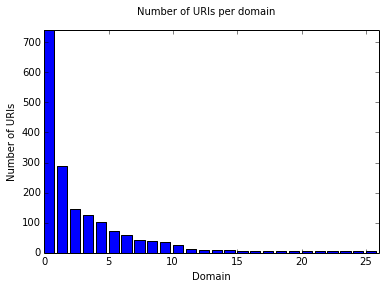
\includegraphics[width=\linewidth]{images/uris_per_domain.png}
      \caption{Total URIs observed at each domain.}
      \label{fig:uris_per_domain:a}
    \end{figure}

    \begin{figure}
      \centering
      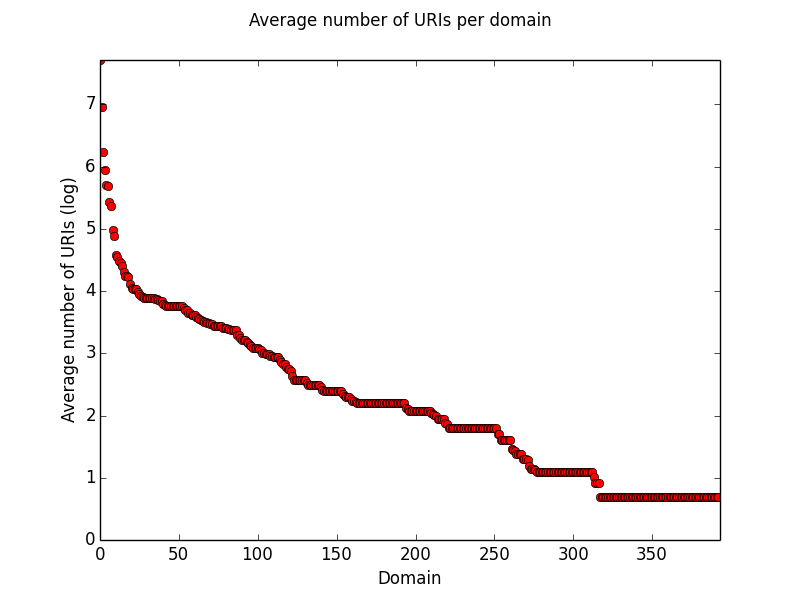
\includegraphics[width=\linewidth]{images/uris_per_domain_avg.png}
      \caption{Average URIs observed at each domain.}
      \label{fig:uris_per_domain:b}
    \end{figure}

    %TODO: These represent a power law relationship between domains and domain size. 
    %TODO: Ignore domain with fewer than 2 pages. What changes?

\section{Experiment: National Archive Collection}

  \begin{enumerate}
  \item Get data from major collection
  \item BL, archive.org, etc.
  \item Apply best strategy from previous section
  \item What real-world savings can we demonstrate?
  \end{enumerate}

\section{Conclusion}

  The defaults in the WARC standard do not take advantage of the fact that many documents on the web will have many minor changes made to them over time. By using a delta algorithm as well as a compression algorithm we can reduce the total archive size by nearly half again.


\end{document}
